\documentclass[12pt,a4paper]{article}
\usepackage{amsmath,amsthm,amsfonts,amssymb,amscd}
\usepackage[T1]{fontenc}
\usepackage{amsfonts}

\usepackage{graphicx}           
% Enhanced support for images
\usepackage{float}              
% Improved interface for floating objects
\usepackage{booktabs}           
% Publication quality tables
\usepackage{xcolor}             
% Driver-independent color extensions
\usepackage[top=3cm, bottom=2.5cm, left=2.5cm, right=2.5cm,
	headsep=0.5cm, headheight=2cm, footskip=1.5cm]{geometry}
% Customize document dimensions
\usepackage{comment}            
% Commenting
\usepackage{adjustbox} 
\usepackage{listings}           
% Typeset programs (programming code) within LaTeX
\usepackage{lastpage}           
% Reference last page for Page N of M type footers.
\usepackage{fancyhdr}           
% Control of page headers and footers
\usepackage{hyperref}           
% Cross-referencing 
\usepackage[small,bf]{caption}  
% Captions
\usepackage{multicol}
\usepackage{tikz}               
% Creating graphic elements
\usepackage{circuitikz}         
% Creating circuits
\usepackage{verbatim}          
% Print exactly what you type in
\usepackage{cite}               
% Citation
\usepackage[us]{datetime} 
% Various time format
\usepackage{blindtext}
% Generate blind text
\usepackage[utf8]{inputenc}
\usepackage{array}
\usepackage{makecell}
\usepackage{tabularx}
\usepackage{titlesec}
\usepackage[italian]{babel}
\usepackage{pgfplots}

\linespread{1.5}

\hypersetup{
    draft=false,
    final=true,
    colorlinks=true,
    citecolor=UM_DarkBlue,
    anchorcolor=yellow,
    linkcolor=UM_DarkBlue,
    urlcolor=UM_DarkBlue,
    filecolor=green,      
    pdfpagemode=FullScreen,
    bookmarksopen=false
    }
    
\definecolor{UM_Brown}{HTML}{3D190D}
\definecolor{UM_DarkBlue}{HTML}{2264B0}
\definecolor{UM_LightBlue}{HTML}{1CA9E1}
\definecolor{UM_Orange}{HTML}{fEB415}

\fancypagestyle{plain}{
	\fancyhf{}
	\rhead{ 
		
\includegraphics[scale=0.05]{figures/PennyWiseLogo.jpeg}
		\textbf{Penny Wise}
		}
	\rfoot{\thepage{} di \pageref{LastPage}}
	\renewcommand{\headrulewidth}{0.2pt}
	\renewcommand{\footrulewidth}{0.2pt}
}
\pagestyle{plain}

\begin{document}
\pagestyle{empty}
\begin{titlepage}
\noindent\makebox[\linewidth]{

\includegraphics[height=6.5cm]{figures/PennyWiseLogo.jpeg}
}
\vspace{15pt}
\textcolor{UM_Brown}{
\begin{flushleft}
    \textbf{\huge{Relazione Progetto Tecnologie Web}}\\
    \vspace{15pt}
    \huge \textbf{Penny Wise} \\
    \vspace{15pt}
	\begin{large}
    \url{http://tecweb.studenti.math.unipd.it/sicaregnato/}
	\newline
    Referente: simone.caregnato@studenti.unipd.it
	\newline
	Credenziali di acesso:
		\begin{itemize}
			\item[] Username: email1@example.com
			\item[] Password: password1
		\end{itemize}
	\end{large}
\end{flushleft}
}
\vspace{55pt}
\textcolor{UM_Brown}{
\begin{flushright}
\begin{tabular}{lcl}
    Basso Leonardo & - & 2042329 \\
    Caregnato Simone & - & 2042884 \\
    Igbinedion Osamwonyi Eghosa Matteo & - & 2042888 \\
    Rosso Carlo & - & 2034293 \\
    Date: &  & \today
\end{tabular}
\end{flushright}
\hrule
}
\end{titlepage}

\newpage
\begin{abstract}
\textit{Penny Wise} è un'idea di Simone Caregnato, nata dalla passione per l'informatica. Questo progetto è stato sviluppato con l'obiettivo di creare due canvas non banali utilizzando esclusivamente JavaScript puro (vanilla JavaScript), come richiesto dai criteri del corso.

L'obiettivo principale del progetto è fornire un'interfaccia semplice e intuitiva per gestire e visualizzare le statistiche delle spese personali. Per rendere il progetto più interessante, è stata aggiunta la funzionalità di condivisione delle spese tra più utenti, permettendo la gestione delle spese comuni, come nel caso di coinquilini.

Le spese possono essere suddivise in categorie, denominate tag, per analizzare la distribuzione delle spese nelle diverse categorie in vari periodi di tempo, offrendo una visione chiara dell'evoluzione delle spese nel tempo.
\end{abstract}
\newpage
\tableofcontents
\newpage
\pagestyle{plain}
\pagenumbering{arabic}
\section{Analisi dei requisiti}

\subsection{Target}

\textit{Grigo Verde} è un servizio dedicato alla gestione delle prenotazioni
delle aree verdi della scuola Michelangelo Grigoletti di Pordenone. Il target
principale è costituito dagli insegnanti della scuola, che necessitano di
strumenti semplici per organizzare le lezioni all'aperto.\\
Il servizio è stato progettato per essere intuitivo e facile da usare, in modo
da permettere agli utenti di prenotare le aree verdi in pochi passaggi. Inoltre,
il servizio è stato progettato per essere accessibile da dispositivi mobili, in
modo da permettere agli utenti di prenotare le aree verdi anche in mobilità.
Considerando il target principale, il servizio è stato progettato per essere
facilmente accessibile e utilizzabile da utenti non esperti di tecnologia.

\subsection{Attori}

Gli attori principali dell'applicazione sono i seguenti:

\begin{itemize}
    \item \textbf{Visitatore}: un utente generico, che non è riconosciuto dal 
        sistema;

    \item \textbf{Utente Docente}: un docente autorizzato, registrato nel
        sistema e che ha effettuato il login;

    \item \textbf{Utente Amministratore}: un amministratore autorizzato,
        registrato nel sistema e che ha effettuato il login.
\end{itemize}

\subsection{Funzionalità}

\textit{Grigo Verde} offre le seguenti funzionalità:
\begin{enumerate}
    \item \textbf{Autenticazione}: login tramite username e password e quindi
    riconoscimento dell'utente da parte del sistema; Disponibile a: 
        \begin{itemize}
            \item Visitatore;
        \end{itemize}

    \item \textbf{Logout}: Disponibile a: 
        \begin{itemize}
            \item Utente docente;
            \item Utente amministratore;
        \end{itemize}

    \item \textbf{Visualizzazione pagina informativa sull'applicazione}, in cui
    viene spiegato lo scopo, le motivazioni delle sua creazione e cosa offre;
    Disponibile a:
        \begin{itemize}
            \item Visitatore;
            \item Utente docente;
            \item Utente amministratore;
        \end{itemize}

    \item \textbf{Visualizzazione degli spazi registrati nel sistema}, con foto
    descrizione, numero di posti; Disponibile a:
        \begin{itemize}
            \item Visitatore;
            \item Utente docente;
            \item Utente amministratore;
        \end{itemize}

    \item \textbf{Filtraggio degli spazi per tipo}, ad esempio per aule o per
    sale ping pong; Disponibile a:
        \begin{itemize}
            \item Visitatore;
            \item Utente docente;
            \item Utente amministratore;
        \end{itemize}

    \item \textbf{Filtraggio degli spazi per disponibilità}, tramite selezione
    del giorno e dell'intervallo temporale; Disponibile a:
        \begin{itemize}
            \item Visitatore;
            \item Utente docente;
            \item Utente amministratore;
        \end{itemize}

    \item \textbf{Visualizzazione delle disponibilità orarie di uno spazio}
    sulla base del mese selezionato; Disponibile a:
    \begin{itemize}
            \item Visitatore; 
            \item Utente docente;
            \item Utente amministratore;
        \end{itemize}

    \item \textbf{Visualizzazione introduzione alle persone che hanno sviluppato
    il progetto}; Disponibile a:
        \begin{itemize}
            \item Visitatore;
            \item Utente docente;
            \item Utente amministratore;
        \end{itemize}

    \item \textbf{Prenotazione di uno spazio disponibile}, specificando il
    giorno da calendario e l'orario; Disponibile a:
        \begin{itemize}
            \item Utente docente;
        \end{itemize}

    \item \textbf{Annullamento prenotazione da lui creata in precedenza};
    Disponibile a:
        \begin{itemize}
            \item Utente docente;
        \end{itemize}

    \item \textbf{Modifica di qualunque prenotazione}: Disponibile a:
        \begin{itemize}
            \item Utente amministratore;
        \end{itemize}

    \item \textbf{Inserimento di prenotazioni periodiche}: inserimento di
    prenotazioni che si ripetono in un intervallo di tempo; Disponibile a:
        \begin{itemize}
            \item Utente amministratore;
        \end{itemize}

    \item \textbf{Creazione di un nuovo spazio}, con inserimento di immagini,
    posizione, nome, tipo, descrizione, numero di tavoli; Disponibile a:
        \begin{itemize}
            \item Utente amministratore;
        \end{itemize}

    \item \textbf{Modifica di uno spazio}: inserimento/eliminazione di immagini,
    modifica posizione, nome, tipo, descrizione, numero di tavoli; Disponibile
    a:
        \begin{itemize}
            \item Utente amministratore;
        \end{itemize}

    \item \textbf{Eliminazione di uno spazio}: Disponibile a:
        \begin{itemize}
            \item Utente amministratore;
        \end{itemize}

    \item \textbf{Inserimento disponibilità spazio}: inserimento in un
    calendario settimanale della disponibilità oraria; Disponibile a:
        \begin{itemize}
            \item Utente amministratore;
        \end{itemize}

    \item \textbf{Creazione di un nuovo tipo di spazio}, con specifica del nome
    e della possibilità o meno di specificare il numero di posti; Disponibile
    a:
    \begin{itemize}
            \item Utente amministratore;
        \end{itemize}

    \item \textbf{Visualizzazione della lista degli utenti registrati nel
    sistema}; Disponibile a:
        \begin{itemize}
            \item Utente amministratore;
        \end{itemize}

    \item \textbf{Registrazione nuovo utente}: aggiunta del nuovo utente al
    sistema con inserimento di nome, cognome, ruolo (docente o amministratore);
    Disponibile a:
        \begin{itemize}
            \item Utente amministratore;
        \end{itemize}

    \item \textbf{Eliminazione utente}: Disponibile a:
        \begin{itemize}
            \item Utente amministratore;
        \end{itemize}

    \item \textbf{Modifica utente}: modifica di nome, cognome e/o ruolo;
    Disponibile a:
        \begin{itemize}
            \item Utente amministratore;
        \end{itemize}
\end{enumerate}

\subsection{SEO}

Innanzitutto, abbiamo immaginao il \textit{search intent} dei nostri utenti. 
Abbiamo identificato le seguenti \textit{query} che potrebbero essere 
utilizzate per cercare il nostro sito:
\begin{itemize}
	\item \textit{Grigo Verde};
	\item \textit{Liceo Grigoletti};
	\item \textit{Liceo Scientifico Pordenone};
	\item \textit{Spazi verdi};
	\item \textit{Aule all'aperto};
\end{itemize}

A partire da queste \textit{query}, abbiamo scritto i tag \texttt{<title>},
\texttt{<meta name="description">} e \texttt{<meta name="keywords">} delle
pagine del nostro sito. Si noti, che queste informazioni non sono aggiunte alle
pagine che richiedono l'autenticazione, in quanto non sono indicizzate dai
motori di ricerca e non sono accessibili ai visitatori non autenticati.\\
Inoltre, sono state adottate soluzioni tecniche, come la
divisione tra la struttura, la presentazione ed il comportamento per ridurre il
peso delle pagine e migliorare il \textit{ranking} nei motori di ricerca. Le
soluzioni tecniche adottate sono spiegate nel dettaglio nelle sezioni dedicate.

\section{Progettazione}

\subsection{Design Persona}

Partendo dalla risorsa consigliata nel corso (\textit{Desining for Emotion} di Aaron Walter), abbiamo descritto la personalità di partenza per sviluppare il prodotto:
\begin{itemize}
    \item \textbf{Brand name}: a questo punto il nome del brand è noto, ovvero
    \textit{Grigo Verde};

    \item \textbf{Overview}: 

    \item \textbf{Brand traits}:
        \begin{itemize}
            \item Formale ma non rigido: deve essere adatto ad un contesto scolastico.
            \item Simpatico ma non scherzoso: questo sito deve essere acceduto da dei docenti, non da bambini di quarta elementare.
            \item Schematico ma non rigido: è vero, è un sistema di prenotazioni, ma è al quanto flessibile.
            \item Preciso: sempre pronto a rispondere ad ogni esigenza dell'utente con la massima accuratezza.
        \end{itemize}
    
    \item \textbf{Personality map}:
        \begin{center}
            \begin{tikzpicture}
                \begin{axis}[
                    axis lines = middle,
                    xlabel = { amichevole },
                    ylabel = { formale },
                    xmin = -10, xmax = 10,
                    ymin = -10, ymax = 10,
                    xtick = {-10,-5,...,10},
                    ytick = {-10,-5,...,10},
                ]
            % template per mostrare il punto all'interno del piano cartesiano.
					\addplot [
						color=black,
						mark=*,
						only marks,
					] coordinates {
					(3, 5)
				} node[below] {$P$};
                \end{axis}
                
            \end{tikzpicture}
        \end{center}

    
    \item \textbf{Voice}: 
		\begin{itemize}
            \item ...
		\end{itemize}
    
    \item \textbf{Copy examples}: ...
    
    \item \textbf{Visual lexicon}:
		\begin{itemize}
			\item \textbf{Colori}: verde scuro per i titoli, nero per i testi e bianco per lo sfondo;  
			\item \textbf{Contorni}: poco arrotondati: la prenotazione delle aule è una procedura precisa. Inserire dei contorni non 
            arrotondati rafforza l'idea di schematico; 
			\item \textbf{Ombre}:assenti;
			\item \textbf{Font}: \textit{Sans-Serif Arial};
            \item ...
		\end{itemize}
    
    \item \textbf{Engagement methods}:
		\begin{itemize}
			\item \textbf{Feedback}: ad ogni azione corriponde una notifica, in
				modo tale che l'utente abbia sempre un riscontro;

			\item \textbf{Design pulito e intuitivo}: l'utente deve essere in
				grado di capire cosa fare senza dover leggere alcun manuale;

			\item \textbf{Psicologia dei colori}: sono utilizzati dei colori
				accattivanti che richiamano il personaggio scelto;

		\end{itemize}
\end{itemize}

\subsection{Palette}

...

\subsection{Accessibilità}

L'accessibilità è un indice di qualità del sito, pertanto è stata fin da subito
un proposito imprescindibile che ha guidato la fase di progettazione e le
successive. Per quanto siamo incorsi in alcune difficoltà. Di seguito sono
riportate le misure adottate per garantire un'esperienza di utilizzo ottimale
per tutti gli utenti.

\subsubsection{Orientamento dell'utente}

\subsubsection{Colori}

I colori sono stati scelti appositamente con un contrasto elevato tra loro in
modo da garantire una buona leggibilità anche da parte di utenti con deficit
parziale della vista, infatti è stato rispettato lo standard WCAG AA.

\subsubsection{Responsive layout}

Il sito è stato progettato per adattarsi a qualsiasi dispositivo, in modo da
garantire un'esperienza di utilizzo ottimale sia da desktop che da mobile. Per
questo motivo, sono stati adottati layout flessibili e fluidi, in modo da
garantire una buona leggibilità e usabilità indipendentemente dalla dimensione
dello schermo o dalle preferenze dell'utente.

\subsection{Struttura del sito}

Il sito è organizzato in una struttura gerarchica per conciliare facilità di
utilizzo e organizzazione delle informazioni in modo ordinato e preciso. I
contenuti sono suddivisi secondo uno schema organizzativo per argomento di
seguito sono descritte le singole pagine:

\begin{itemize}
    \item ...
\end{itemize}

\section{Realizzazione}

\subsection{Back-end}

\subsubsection{Database}

\begin{figure}[H]
	\centering
	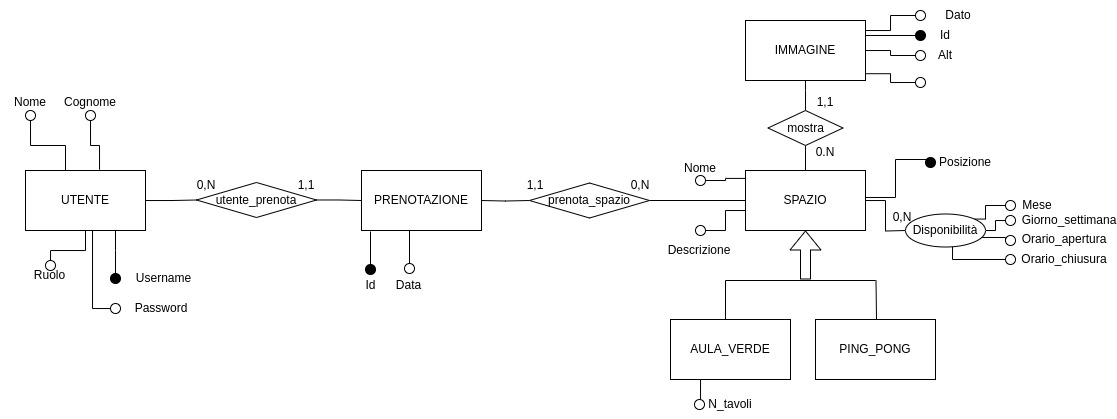
\includegraphics[width=0.9\textwidth]{figures/Database}
	\caption{Diagramma del database}
\end{figure}

Per stabilire la connessione con il database viene utilizzata l'estensione
\texttt{MySQLi} di PHP.

\subsection{Front-end}

\section{Test}
\label{sec:test}

Per controllare la qualità di Grigo Verde sono eseguiti diversi test:
\begin{itemize}
	\item Test di unità: per controllare la business logic abbiamo creato una
	      pagina html che invoca delle funzioni di test in php durante la
	      creazione della pagina. Per accedere alla pagina dei test, bisogna
	      rimuovere il commento alla riga 42 del file
	      \texttt{GrigoVerde/src/controller/routes.php}; finalmente è
	      sufficiente accedere alla pagina \texttt{test} a partire dal base url
	      del sito;

	\item Test mediante l'estensione browser Wave: per controllare
	      l'accessibilità in modo automatico;

	\item Test mediante Total Validator: per controllare l'accessibilità in modo
	      automatico;

	\item Test mediante il validatore W3C: per controllare la validità del codice
	      HTML e CSS;

	\item Test manuali: per controllare l'accessibilità in modo manuale;

	\item Test di usabilità: per controllare l'usabilità del sito, anche su
	      dispositivi di diverse dimensioni;

	\item Test di compatibilità: per controllare la compatibilità con i browser
	      più diffusi;

	\item Test sul contrasto dei colori: per controllare che il contrasto dei
	      colori sia sufficiente per garantire l'accessibilità a persone con
	      disabilità visive con Adobe Color.
\end{itemize}

Non abbiamo rilevato errori con i test automatici, mentre con i test manuali
abbiamo riscontrato che il sito è accessibile e usabile.

\section{Organizzazione del lavoro}

\subsection{Basso Leonardo}
\begin{itemize}
	\item Definizione del database;

	\item Sviluppo del comportamento del client, ovvero di tutto il codice che
		viene scritto in JavaScript e che viene eseguito sul browser 
		dell'utente;

	\item \textit{Proof of concept} del Model;
\end{itemize}

\subsection{Caregnato Simone}
\begin{itemize}
	\item Sviluppo del Model;
	\item Popolamento del database;
	\item Sviluppo di \texttt{CakeChart}, ovvero del codice JavaScript che si 
		occupa di disegnare i grafici a torta;
	\item Testing delle funzionalità nel client;
\end{itemize}

\subsection{Igbinedion Osamwonyi Eghosa}
\begin{itemize}
	\item Sviluppo della presentazione del client, ovvero tutto il codice CSS;
	\item Correzione dell'HTML;
	\item Testing dell'accessibilità del client;
\end{itemize}

\subsection{Rosso Carlo}
\begin{itemize}
	\item Sviluppo della struttura del client, ovvero di tutto il codice HTML;
	\item Sviluppo di \texttt{LineChart}, ovvero del codice JavaScript che si 
		occupa di disegnare i grafici a linee;
	\item Sviluppo del Controller;
\end{itemize}


\end{document}

% \subsection{SEO}
% 
% Innanzitutto, abbiamo immaginao il \textit{search intent} dei nostri utenti.
% Abbiamo identificato le seguenti \textit{query} che potrebbero essere
% utilizzate per cercare il nostro sito:
% \begin{itemize}
% 	\item \textbf{Grigo Verde};
% 	\item \textbf{Liceo Grigoletti};
% 	\item \textbf{Liceo Scientifico Pordenone};
% 	\item \textbf{Spazi verdi};
% 	\item \textbf{Aule all'aperto};
% \end{itemize}
% 
% A partire da queste \textit{query}, abbiamo scritto i tag \texttt{<title>},
% \texttt{<meta name="description">} e \texttt{<meta name="keywords">} delle
% pagine del nostro sito. Si noti, che queste informazioni non sono aggiunte alle
% pagine che richiedono l'autenticazione, in quanto non sono indicizzate dai
% motori di ricerca e non sono accessibili ai visitatori non autenticati. In
% aggiunta, sono state aggiunte keyword specifiche per ogni pagina, in modo da
% migliorare il posizionamento nei motori di ricerca.\\
% Finalmente, sono state adottate soluzioni tecniche, come la
% divisione tra la struttura, la presentazione ed il comportamento per ridurre il
% peso delle pagine e migliorare il \textit{ranking} nei motori di ricerca. Le
% soluzioni tecniche adottate sono spiegate nel dettaglio nelle sezioni dedicate.
